\documentclass[letterpaper,11pt,oneside,reqno]{article}

%%%%%%%%%%%%%%%%%%%%%%%%%%%%%%%%%%%%%%%%%%%%%%%%%%%%%%%%%%%%

\usepackage[pdftex,backref=page,colorlinks=true,linkcolor=blue,citecolor=red]{hyperref}
\usepackage[alphabetic,nobysame]{amsrefs}

%%%%%%%%%%%%%%%%%%%%%%%%%%%%%%%%%%%%%%%%%%%%%%%%%%%%%%%%%%%%
%main packages
\usepackage{amsmath,amssymb,amsthm,amsfonts,mathtools}
\usepackage{graphicx,color}
\usepackage{upgreek}
\usepackage[mathscr]{euscript}

%equations
\allowdisplaybreaks
\numberwithin{equation}{section}

%tikz
\usepackage{tikz}
\usetikzlibrary{shapes,arrows,positioning,decorations.markings}

%conveniences
\usepackage{array}
\usepackage{adjustbox}
\usepackage{cleveref}
\usepackage{enumerate}
\usepackage{datetime}

%paper geometry
\usepackage[DIV=12]{typearea}

%%%%%%%%%%%%%%%%%%%%%%%%%%%%%%%%%%%%%%%%%%%%%%%%%%%%%%%%%%%%
%draft-specific
\synctex=1
% \usepackage{refcheck,comment}

%%%%%%%%%%%%%%%%%%%%%%%%%%%%%%%%%%%%%%%%%%%%%%%%%%%%%%%%%%%%
%this paper specific
\newcommand{\ssp}{\hspace{1pt}}

%%%%%%%%%%%%%%%%%%%%%%%%%%%%%%%%%%%%%%%%%%%%%%%%%%%%%%%%%%%%
\newtheorem{proposition}{Proposition}[section]
\newtheorem{lemma}[proposition]{Lemma}
\newtheorem{corollary}[proposition]{Corollary}
\newtheorem{theorem}[proposition]{Theorem}
%%%%%%%%%%%%%%%%%%%%%%%%%%%%%%%%%%%%%%%%%%%%%%%%%%%%%%%%%%%%
\theoremstyle{definition}
\newtheorem{definition}[proposition]{Definition}
\newtheorem{remark}[proposition]{Remark}
%%%%%%%%%%%%%%%%%%%%%%%%%%%%%%%%%%%%%%%%%%%%%%%%%%%%%%%%%%%%

\begin{document}
\title{Lectures on Random Matrices
(Spring 2025)
\\Lecture 13: Matching a Random Matrix Model to a Random Growth Model}


\date{Wednesday, April 9, 2025\footnote{\href{https://lpetrov.cc/rmt25/}{\texttt{Course webpage}}
$\bullet$ \href{https://lpetrov.cc/simulations/model/random-matrices/}{\texttt{Live simulations}}
$\bullet$ \href{https://lpetrov.cc/rmt25/rmt25-notes/rmt2025-l13.tex}{\texttt{TeX Source}}
$\bullet$
Updated at \currenttime, \today}}



\author{Leonid Petrov}


\maketitle

\section{Recap}

In the last lecture, we discussed various random growth models, and universal KPZ objects:
\begin{itemize}
	\item \textbf{Airy line ensemble} which arises as the scaling limit of the Dyson Brownian motion.
	\item \textbf{KPZ Equation} as a universal continuous random growth model.
	\item \textbf{Polynuclear growth model} (PNG) as a discrete analogue of the KPZ equation.
\end{itemize}

Then we briefly mentioned how the PNG model matches to a
last-passage percolation (LPP) model in
$\mathbb{R}^2_{\ge0}$ driven by the Poisson
point process as noise.
In this lecture, we are going to explore a different
LPP model which is defined on cells of $\mathbb{Z}_{\ge1}^{2}$, and
match it \emph{exactly} to the Wishart random matrix model which we have seen before in passing.
This matching is due to Dieker and Warren (2009)
\cite{dieker2008largest}, who proved it
in the context
of deformed random matrix spectra,
as suggested in
\cite{BorodinPeche2009}.
The key to this matching is a \emph{dynamical} perspective
on both the LPP and the random matrix models, which allows us to
match Markov chains in the two models, and not simply the distributions.

Throughout the discussion, we will consider the ``spiked'', multiparameter models,
which naturally include finite-rank deformations.

\section{The spiked Wishart ensemble}
\label{sec:Wishart}

\subsection{Definition of the spiked Wishart process}
\label{sub:Wishart_process}

Recall that a (complex) \emph{Wishart matrix} $M$ of dimension
$n$ with $t$ degrees of freedom (and identity covariance)
can be represented as $M = X X^*$, where $X$ is an $n\times
t$ random matrix with independent complex Gaussian entries.
Clearly, $M$ is a positive-semidefinite Hermitian matrix of
size $n\times n$. The eigenvalues
$(\lambda_1,\dots,\lambda_N)$ (with $\lambda_1\ge \cdots \ge
\lambda_N \ge 0$) have the joint density of the
\emph{Laguerre orthogonal polynomial ensemble} ($\beta=2$).
Now we introduce a more
general model where the covariance of the underlying
Gaussian matrix is not identity but has a
perturbation (a ``spike'').

\begin{definition}[Generalized Wishart ensemble with parameters $(\pi,\hat\pi)$]\label{def:Wishart}
Fix a positive integer $n$. Let $\pi=(\pi_1,\dots,\pi_n)$ be a fixed $n$-tuple of \emph{positive} real parameters, and let $\hat\pi = (\hat\pi_1,\hat\pi_2,\dots)$ be a sequence of \emph{nonnegative} real parameters (possibly infinite in length). We define an array of complex random variables $\{A_{ij}: 1\le i\le n, j\ge 1\}$ such that under the probability measure $P^{\pi,\hat\pi}$:
\begin{itemize}\item The $A_{ij}$ are independent for all $1\le i\le n$ and $j\ge 1$.
\item Each $A_{ij}$ is a complex Gaussian with mean $0$ and variance $\mathrm{Var}(A_{ij}) = \frac{1}{\pi_i + \hat\pi_j}$ (i.e. $\Re A_{ij}, \Im A_{ij} \sim N(0,\frac{1}{2(\pi_i+\hat\pi_j)})$ independent).
\end{itemize}
For each integer $t\ge 0$, let $A(t)$ denote the $n\times t$ sub-matrix consisting of the first $t$ columns of $A$. We then define an $n\times n$ random Hermitian matrix
\[ M(t) := A(t)\,A(t)^*, \qquad t\ge 0, \]
with the convention $M(0)$ is the zero matrix. We call $\{M(t): t\ge 0\}$ the \textbf{generalized Wishart random-matrix process} with parameters $(\pi,\hat\pi)$.
\end{definition}

In particular, $M(t)$ has the form
\[ M(t) = \sum_{m=1}^t A^{(m)} (A^{(m)})^*, \]
where $A^{(m)}$ denotes the $m$-th column of $A$ (an
$n$-dimensional complex random vector with independent
entries of variance $1/(\pi_i+\hat\pi_m)$). When all $\pi_i=1$ and all
$\hat\pi_j=0$, $M(t)$ reduces to the classical complex
Wishart($n,t$) with identity covariance.

\begin{remark}
	The introduction of parameters $\pi$ and $\hat\pi$ allows
	for \textbf{finite-rank deformations of the covariance}: one
	can think of the $\pi_i$'s as baseline values (say $\pi_i=1$
	for all but a few coordinates), and a finite number of them
	being different from 1 corresponds to a finite-rank
	perturbation of the identity covariance matrix $\Sigma$ (the
	directions in which $\pi_i\neq 1$ are "spiked"
	eigen-directions). Similarly, $\hat\pi_j$ can be viewed as
	adding a rank-one perturbation associated with each column;
	if only finitely many of the $\hat\pi_j$ are nonzero, that
	corresponds to having a finite number of distinguished
	samples (or boundary inhomogeneities in the equivalent
	percolation model, as we will see).
\end{remark}

We emphasize that $M(t)$
depends on $t$ in a way that $M(t)$ and $M(t-1)$ are not
independent but are coupled through shared columns. Indeed
$M(t) = M(t-1) + A^{(t)}(A^{(t)})^*$, which is a rank-1
update of $M(t-1)$.

\medskip
Let us denote by $\lambda_1(t)\ge \lambda_2(t)\ge \cdots \ge
\lambda_n(t)\ge 0$ the eigenvalues of $M(t)$ in
non-increasing order (padded with zeros if $t < n$, since
$\mathrm{rank}(M(t)) \le t$). We will use the notation
$\operatorname{sp}(M(t)) =
(\lambda_1(t),\dots,\lambda_n(t))$ for the \emph{spectrum}
of $M(t)$, viewed as a vector in the \emph{Weyl chamber}
$\mathbb{W}^n = \{x=(x_1,\dots,x_n)\in\mathbb{R}^n: x_1 \ge x_2 \ge
\cdots \ge x_n\}$. We are particularly interested in the
\emph{largest eigenvalue process}
$\{\lambda_1(t):t\ge0\}$, i.e. the sequence of the top
eigenvalue as the number of samples $t$ grows. Our goal is
to describe the law of this process and to identify it with
a combinatorial growth model.

Before stating the main result, we need a fundamental
property of the eigenvalue sequence
$\operatorname{sp}(M(t))$ as $t$ increases, namely that it
forms a \emph{Markov chain} in $\mathbb{W}^n$.
See Problem~\ref{prob:Markov}.

We need another statement:
\begin{lemma}[Interlacing; Problem~\ref{prob:interlacing}]
\label{lemma:interlacing}
For each $t\geq 1$, the eigenvalues of $M(t)$ and $M(t-1)$ satisfy the interlacing property:
\begin{equation}
	\label{eq:interlace}
	\lambda_1(t) \geq \lambda_1(t-1) \geq \lambda_2(t) \geq \lambda_2(t-1) \geq \cdots \geq \lambda_n(t-1) \geq \lambda_n(t) \geq 0.
\end{equation}
\end{lemma}
We denote the relation \eqref{eq:interlace} by
\begin{equation}
	\label{eq:interlace-notation}
	\lambda(t) \succ \lambda(t-1).
\end{equation}

In other words, the eigenvalue \emph{Markov processes}
$\lambda(t)$, $t=0,1,2,\ldots $
form an interlacing array, where at each step of the Markov process,
a new row of the array is ``revealed''.
The interlacing property is parallel to
the uniform conditioning (Gibbs) property in the $\beta=2$ corners. Moreover,
one can check (Problem~\ref{prob:Gibbs}) that
in the null case
$\pi_i=1$ and $\hat\pi_j=0$,
the Wishart eigenvalue process satisfies the
uniform Gibbs property as well.

\subsection{Markov chain and transition kernel for eigenvalues}
We say a random process $\{X(t):t\ge0\}$ taking values in
$\mathbb{W}^n$ is an \emph{inhomogeneous Markov chain} if
for each $m<t$, the conditional law of $X(t)$ given
$(X(t-1)=x_{t-1},\;X(t-2)=x_{t-2},\dots,X(m)=x_m)$ depends
only on $x_{t-1}$ (and possibly on $t$). In other words, the
process has the Markov property but the transition kernel
may depend on the time step $t$. In our case, since at each
step $t$ a new column $A^{(t)}$ with variance parameters
$\{\pi_i+\hat\pi_t:1\le i\le n\}$ is added, the transition
law from $M(t-1)$ to $M(t)$ will indeed depend on the index
$t$ through $\hat\pi_t$. We denote by
$Q^{\pi,\hat\pi}_{t-1,t}(x,dy)$ the transition kernel: for
$x\in \mathbb{W}^n$ given as the eigenvalue vector of
$M(t-1)$, $Q^{\pi,\hat\pi}_{t-1,t}(x,\cdot)$ is the
distribution of $\operatorname{sp}(M(t))$.

The null case $\pi_i=1$ and $\hat\pi_j=0$ of $Q^{\pi,\hat\pi}_{t-1,t}(x,dy)$
was computed in \cite{defosseux2010orbit}, see also
\cite{forrester2006jacobians}.

\begin{theorem}
\label{thm:MarkovChain}
Fix an integer \(n\ge1\).  Let \(\pi=(\pi_1,\dots,\pi_n)\) be a strictly positive \(n\)-vector, and let \(\widehat\pi=(\widehat\pi_1,\widehat\pi_2,\dots)\) be any sequence of nonnegative real parameters.  Under the probability measure \(P^{\pi,\widehat\pi}\), the eigenvalues of the \(n\times n\) generalized Wishart matrices \(\{M(t)\}_{t\ge0}\) form a time-inhomogeneous Markov chain \(\{\mathrm{sp}(M(t))\}_{t\ge0}\) in the Weyl chamber
\[
\mathbb{W}^n
\;=\;
\bigl\{\,x=(x_1,\dots,x_n)\in\mathbb{R}^n_{\ge0}:
x_1\ge x_2\ge\cdots\ge x_n\bigr\}.
\]
More precisely, writing \(x=\mathrm{sp}(M(t-1))\) and \(y=\mathrm{sp}(M(t))\), the one-step transition law from time \((t-1)\) to \(t\) is absolutely continuous on the interior of \(\mathbb{W}^n\) and can be factored as
\begin{equation}
\label{eq:transition-density}
Q_{t-1,t}^{\pi,\widehat\pi}(x,\,dy)
\;=\;
\Bigl[\,
\prod_{i=1}^n \bigl(\pi_i+\widehat\pi_{t}\bigr)
\Bigr]
\cdot
\frac{h_{\pi}(y)}{h_{\pi}(x)}
\;\exp\Bigl(-(\widehat\pi_{t}-1)\sum_{i=1}^n (y_i - x_i)\Bigr)
\;\times\;Q^{(0)}\bigl(x,\,dy\bigr),
\end{equation}
where
\begin{itemize}
\item \(\displaystyle Q^{(0)}\bigl(x,\,dy\bigr)\) is the \emph{standard} (null-spike) Wishart transition kernel, given explicitly by
	\begin{equation}
		\label{eq:Q0}
Q^{(0)}(x,\,dy)
\;=\;
\frac{\Delta(y)}{\Delta(x)}\;\exp\Bigl(\,-\sum_{i=1}^n (y_i - x_i)\Bigr)\,
\mathbf{1}_{\{x\prec y\}}\;dy,
\end{equation}
with \(\Delta(z)=\prod_{1\le i<j\le n}(z_i - z_j)\) the Vandermonde determinant.

\item The function \(h_{\pi}\) is the (continuous) Harish-Chandra orbit integral factor
\[
h_{\pi}(z)
\;=\;
\frac{(-1)^{\binom n2}}{0! 1! \cdots (n-1)! }
\frac{\det\bigl(e^{-\pi_i\,z_j}\bigr)_{i,j=1}^n}{\Delta(\pi)\,\Delta(z)}.
\]
Note that $h_\pi(0)=1$.
\end{itemize}
In particular, the chain starts from \(\mathrm{sp}(M(0))=0\) (the zero matrix).
\end{theorem}

\begin{proof}[Sketch of proof; see \cite{dieker2008largest}]
	First of all, random-matrix arguments
	\cite{defosseux2010orbit}, \cite{forrester2006jacobians} show that the
	theorem holds for the null case $\pi_i=1$ and $\hat\pi_j=0$.
	The Radon-Nikodym derivative of the transition kernel
	factors through the diagonal entries of the matrix,
	and can be written in terms of the eigenvalues via
	the HCIZ integral.
	This yields an explicit factor multiplying the null-case
	transition density.
\end{proof}



\begin{remark}[Problem~\ref{prob:CauchyBinet}]
\label{rem:CauchyBinet}
In order to see directly that the family $\bigl\{Q^{\pi,\hat{\pi}}_{t-1,t}\bigr\}$ of transition kernels does indeed define Markov transitions (that is, each $Q^{\pi,\hat{\pi}}_{t-1,t}(x,\cdot)$ is a probability measure for every $x$), one can use the fact that
\[
	\mathbf{1}_{z \prec z'}
\;=\;
\det\bigl[\mathbf{1}_{z_i < z'_j}\bigr],
\]
along with the Cauchy--Binet (or Andr\'eief) identity:
\[
\int_{\mathbb{W}^N}
\det[\xi_i(z_j)]\,
\det[\psi_j(z_i)]
\,dz
\;=\;
\det\Bigl[
\int_{\mathbb{R}}
\xi_i(z)\,\psi_j(z)\,dz
\Bigr].
\]
Applying this to
\eqref{eq:transition-density}--\eqref{eq:Q0}
yields an integral over the Gelfand--Tsetlin polytope
of certain exponential weights, which yields something like $h_{\hat \pi}(y)$.
Then, using Andr\'eief's identity, we need to integrate
exponential densities of the form $e^{-(\pi_i+\hat \pi_j)y}$.
Finally, the determinant of $\dfrac{1}{\pi_i+\hat \pi_j}$ is the Cauchy determinant,
and yields the normalizing factor
$\prod_{i,j}(\pi_i+\hat \pi_j)$.
This should
confirm that each transition kernel
integrates to one, in line with the notation and
factorization in Theorem~\ref{thm:MarkovChain}.
\end{remark}

The fixed-time distribution of the eigenvalues
in the null case $\pi_i=1$ and $\hat\pi_j=0$ is
given by the Laguerre orthogonal polynomial ensemble. For example, for $t\ge n$, we have
\begin{equation}
	\label{eq:Laguerre}
	\operatorname{Prob}(\operatorname{sp}(M(t))\in dy)
	=
	\frac{1}{Z}\prod_{i<j}(y_i-y_j)^2
	\prod_{i=1}^n y_i^{t-n} e^{-y_i}.
\end{equation}
For the non-null case, see Problem~\ref{prob:Wishart_non_null}.

\section{The lattice LPP model}

\subsection{Definition of the model}

We now turn to a seemingly different probabilistic model: a
model of random paths in a grid with random weights. Fix an
integer $n$. Consider an infinite array of independent,
nonnegative random weights $\{W_{ij}: 1\le i\le n,\; j\ge
1\}$ defined under the probability measure $P^{\pi,\hat\pi}$,
where each $W_{ij}$ is an independent random variable with
an \emph{exponential} distribution of rate $(\pi_i +
\hat\pi_j)$.
Note that $\mathbb{E}[W_{ij}] = \frac{1}{\pi_i+\hat\pi_j}$.
These rates $(\pi_i+\hat\pi_j)$ are chosen deliberately to
mirror the variance parameters of $A_{ij}$ in the
generalized Wishart model (Definition \ref{def:Wishart}).

We interpret $\{W_{ij}\}$ as random weights on the vertices of a directed lattice in the first quadrant. Specifically, consider the set of lattice points
\[ \{(i,j): i=1,\dots,n,\ j=1,2,\dots\}.\]
We say a path $\Gamma$ is an \emph{up-right path} from
$(1,1)$ to $(n,t)$ if it is a sequence of lattice points
starting at $(1,1)$ and ending at $(n,t)$, with steps either
one step to the right or one step down. Since each step
either increases the column index by 1 or the row index by
1, any such path from $(1,1)$ to $(n,t)$ must consist of
$(n-1)$ down-steps and $(t-1)$ right-steps, for a total of
$(n+t-2)$ steps. We define the \emph{weight} of a path
$\Gamma$ to be the sum of the $W_{ij}$ along its vertices:
\[ \mathcal{W}(\Gamma) := \sum_{(i,j)\in \Gamma} W_{ij}, \]
where by $(i,j)\in \Gamma$ we mean that the vertex $(i,j)$ is visited by the path $\Gamma$. The random variable of interest is the \emph{maximum total weight achievable among all such paths}, i.e.
\begin{equation}\label{eq:LPPdef}
Y(n,t) := \max_{\Gamma:\, (1,1)\to(n,t)} \; \mathcal{W}(\Gamma)\,.
\end{equation}
We call $Y(n,t)$ the \emph{last-passage time} to $(n,t)$, in analogy with the usual terminology of growth models (if we interpret $W_{ij}$ as random passage times on a lattice, then the longest time to reach a certain site is given by the maximal weight path).

\begin{figure}[ht]
\centering
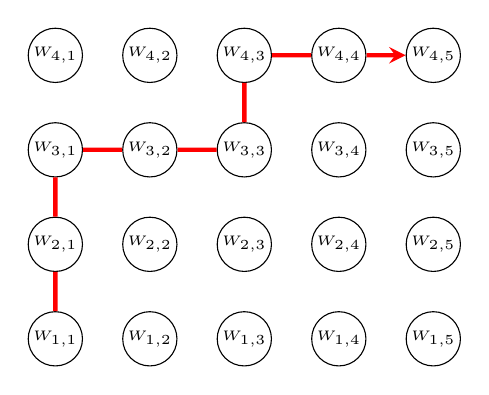
\begin{tikzpicture}[scale=1.2,>=stealth]
    % Draw a 4 (rows) by 5 (columns) grid of nodes.
    % We'll place row i = 1 at the bottom and i = 4 at the top,
    % and columns j=1..5 from left to right.
    % Each node is labeled with W_{i,j}.
    \foreach \i in {1,2,3,4} {
        \foreach \j in {1,2,3,4,5} {
            % Position nodes so that i=1 is bottom row, i=4 top row.
            \node[circle,draw,fill=white,inner sep=1pt]
                  (n\i-\j)
                  at (\j,\i)
                  {\tiny $W_{\i,\j}$};
        }
    }

    % Draw one example of an up-right path from (1,1) to (4,5).
    % It has exactly 3 "up" steps (increasing i) and 4 "right" steps (increasing j).
    \draw[ultra thick, red,->]
        (n1-1) -- (n2-1) -- (n3-1) -- % three steps up
        (n3-2) -- (n3-3) --           % two steps right
        (n4-3) --                     % one step up
        (n4-4) -- (n4-5);             % two steps right

    % Optionally, you can add arrows for all edges (to the right and upward)
    % if you want to depict the entire directed lattice structure.
    % E.g.:
    % \foreach \i in {1,...,4}{
    %   \foreach \j in {1,...,4}{
    %       \draw[->,black!30] (n\i-\j) -- (n\i-\the\numexpr\j+1\relax);
    %   }
    % }
    % \foreach \i in {1,...,3}{
    %   \foreach \j in {1,...,5}{
    %       \draw[->,black!30] (n\i-\j) -- (n\the\numexpr\i+1\relax-\j);
    %   }
    % }
\end{tikzpicture}
\caption{A portion of the lattice with vertex-weights $W_{i,j}$ and one up-right path.}
\end{figure}


Indeed, it is immediate from the definition that the random
variables $Y(n,t)$ satisfy the following random recursion:
\begin{equation}\label{eq:LPP-recursion}
Y(i,j) = W_{ij} + \max\{\, Y(i-1,j),\; Y(i,j-1)\,\}\,,
\end{equation}
for $i>1, j>1$, with boundary conditions $Y(1,j) =
\sum_{k=1}^j W_{1k}$ and $Y(i,1) =
\sum_{\ell=1}^i W_{\ell,1}$.
The recursion \eqref{eq:LPP-recursion} expresses
that the optimal path to $(i,j)$ either comes from above
(then last step is down, contributing $W_{ij}$ plus the
optimal weight to $(i-1,j)$) or from the left (last step is
right from $(i,j-1)$). It is the fundamental equation of
integrable growth models, which is a part of the
\emph{Robinson--Schensted--Knuth insertion algorithm} in
combinatorics. 


\begin{remark}
The quantity $Y(n,t)$ appears in many contexts: it is the
length of the longest increasing path in a random $n\times
t$ array (if $W_{ij}$ were thought of as lengths or as
indicator of a path's presence), it is also the total
service time in a series of $n$ exponential queueing servers
with $t$ customers (the \emph{Jackson network}
interpretation \cite{Baryshnikov_GUE2001}), and it is a
prototype of models in the KPZ universality class (often
called the \emph{exponential corner growth model} or
directed percolation). Standard references on the
connections between random matrices and such growth models
include Baryshnikov (2001) \cite{Baryshnikov_GUE2001} and
Johansson (2000) \cite{Johansson2000}. In particular, when
all $\pi_i=1$ and $\hat\pi_j=0$ (the homogeneous case where
all $W_{ij}\sim \mathrm{Exp}(1)$ i.i.d.), it is known that
$Y(n,t)$ (for large $n,t$ with $n/t$ fixed) has fluctuations
of order $n^{1/3}$ and converges to the Tracy--Widom GUE
distribution after centering and scaling
\cite{Johansson2000}. This is the same limiting law as the
largest eigenvalue of an $n\times n$ GUE matrix. In fact,
Baryshnikov \cite{Baryshnikov_GUE2001} showed that for the
homogeneous case, the entire sequence $\{Y(k,t):1\le k\le
n\}$ (for fixed $t$) has the same distribution as the
ordered eigenvalues $(\lambda_1,\dots,\lambda_n)$ of an
$n\times n$ GUE (Gaussian unitary ensemble) matrix. This was
one of the first precise links between random matrix spectra
and last-passage percolation. In our present setting, the
weights are not identically distributed but have rates
$\pi_i+\hat\pi_j$, which introduces a spatial inhomogeneity
(often called \emph{boundary deformation} of the LPP model).
As we will see, even in this deformed case, one can relate
the LPP times to random matrix eigenvalues --- in fact,
exactly to the spiked Wishart eigenvalues introduced in 
\Cref{sec:Wishart}.
\end{remark}

Let us define the whole \emph{vector of last-passage times to the bottom row} at column $j$ as
\[ Z(j) := \big( Y(1,j),\, Y(2,j),\, \dots,\, Y(n,j)\big)\,\in W^n, \]
where we list the values in increasing order $Y(1,j)\le Y(2,j)\le \cdots \le Y(n,j)$.\footnote{We have $Y(1,j)\le \cdots\le Y(n,j)$ almost surely because giving the path more freedom to move down can only increase the maximum weight. This is easily checked from \eqref{eq:LPP-recursion}. Thus $Z(j)\in W^n$ indeed.} In particular, $Y(n,t)$ is the largest component of $Z(t)$. The sequence $\{Z(t):t\ge0\}$, with $Z(0)=(0,\dots,0)$, is a random process in $W^n$. We will now describe how the RSK correspondence shows that $Z(t)$ is an inhomogeneous Markov chain and, crucially, has the \emph{same transition kernel} as the eigenvalue chain $\operatorname{sp}(M(t))$ from Section 2. This will pave the way to prove the equality in distribution.

\subsection{The Robinson--Schensted--Knuth (RSK) correspondence}
The RSK algorithm is a combinatorial bijection that associates to any matrix of nonnegative integers a pair of Young Tableaux of the same shape. We refer to standard texts (e.g. Fulton \cite{fulton1997young}) for background on Young Tableaux and the classical (unweighted) RSK correspondence. Here we will use a more probabilistic perspective suitable for our random weights. Specifically, RSK can be described as a procedure that takes an $N\times n$ array of weights (for example $W_{ij}$ for $1\le i\le N,\,1\le j\le n$) and outputs a \textbf{Gelfand--Tsetlin (GT) pattern} of depth $N$ and width $n$. A GT pattern of depth $N$ is a triangular array $x=(x_i^k)_{1\le i\le k \le N}$ of real numbers with $k$ entries in row $k$, satisfying the interlacing constraints
\[ x^k_i \;\ge\; x^{k-1}_i \;\ge\; x^k_{i+1} \qquad \text{for each $1\le i < k \le N$.} \]
We denote by $\mathcal{GT}_{N}$ the set of all GT patterns with $N$ levels. It is well-known that there is a bijection between $\mathcal{GT}_N$ and the set of pairs of \emph{semi-standard Young Tableaux} of a certain shape with entries in $\{1,\dots,N\}$ (the shape is given by the bottom row of the GT pattern). In fact, the classical RSK correspondence says that if $(P,Q)$ is the pair of SSYTs associated with the matrix, then the shape $\lambda$ (a partition of some integer) satisfies $\lambda_1 = Y(N,n)$, $\lambda_2 = Y(N-1,n)$, ..., $\lambda_N = Y(1,n)$, where $Y(k,n)$ are exactly the LPP times defined earlier (this is a consequence of Greene's theorem, which generalizes the Schensted theorem on longest increasing subsequences to the case of $k$ disjoint increasing subsequences) \cite{Greene1974, fulton1997young}. In other words, the shape of the tableau (or equivalently the bottom row $(x^N_1,\dots,x^N_N)$ of the GT pattern) is precisely the sorted vector of last-passage times to $(k,n)$ for $k=1,\dots,N$. Thus we have:
\begin{equation}\label{eq:RSK-property}
x^N_i(n) \;=\; Y(i,n)\qquad \text{for $i=1,\dots,N$},
\end{equation}
where we use the notation $x^N_i(n)$ to denote the $i$-th entry of the bottom row of the GT pattern produced by applying RSK to the submatrix of weights $\{W_{ij}: 1\le i\le N, 1\le j\le n\}$.

In our context, the $W_{ij}$ are not integers a.s., but the RSK algorithm can be extended to real-valued matrices as well, by an appropriate limiting procedure. Essentially, one can approximate the $W_{ij}$ by rationals or by increments of small integers and apply the discrete RSK, then take a limit (this is sometimes called the \emph{greedy algorithm} or \emph{greene's algorithm} for continuous input). For our purposes, we take \eqref{eq:RSK-property} as the defining property linking the LPP values to the GT pattern generated by RSK. Equation \eqref{eq:RSK-property} is precisely the statement of (the weighted version of) Greene's theorem: it asserts that the maximum weight of an up-right path that uses $i$ down-steps (i.e. reaches row $i$) is equal to the $i$-th smallest entry in the RSK output shape. For completeness, we note that in the unweighted case ($W_{ij}=1$ for all entries in some submatrix), $Y(i,n)$ would simply be the length of the longest path using $i$ down-steps, which is exactly the length of the $i$-th longest increasing subsequence of a corresponding sequence --- Greene's theorem then says this equals the sum of the first $i$ parts of the Young diagram (the shape's first $i$ row lengths), which recovers the Schensted correspondence in the case $i=1$.

Now, a crucial property of RSK is that it is a \emph{bijection}. This means that given the output GT pattern, one can reconstruct the input matrix (or rather, the multiset of input entries). In particular, if we feed in a random matrix $\{W_{ij}:1\le i\le N, 1\le j\le n\}$, the distribution of the output pattern $X(n)\in \mathcal{GT}_N$ (where $X(n)$ denotes the GT pattern after processing $n$ columns of the matrix) can be characterized by this bijectivity. For example, suppose $W_{ij}$ are geometric random variables taking values in $\mathbb{Z}_{\ge0}$ (the discrete analogue of our exponential weights). Specifically, assume each $W_{ij}$ is independent with $\mathbb{P}\{W_{ij}=k\} = (1-a_i b_j) (a_i b_j)^k$ for $k\in\{0,1,2,\dots\}$, where $0<a_i, b_j <1$ are parameters. This is a geometric distribution with mean $\frac{a_i b_j}{1-a_i b_j}$. In the special case $a_i = a$ for all $i$ and $b_j=b$ for all $j$, such a model is equivalent (after a certain mapping) to the totally asymmetric simple exclusion process (TASEP) with certain initial conditions, and RSK provides a coupling to the Poissonized Plancherel measure (see \cite{OConnell2003}). In our more general case with distinct $a_i, b_j$, the distribution of the GT pattern $X(n)$ can be described by known results: it turns out that \emph{the bottom row of the GT pattern $X(n)$ evolves as an inhomogeneous Markov chain in $W^N$ with an explicit transition probability depending on $a_i, b_j$}. Indeed, the following proposition is essentially proved by O'Connell \cite{OConnell2003}:

\begin{proposition}[Markov property of LPP via RSK]\label{prop:RSK-Markov}
Apply the RSK algorithm column-by-column to the infinite array of geometric random variables $\{\xi_{ij}: 1\le i\le N,\ j\ge1\}$ with $\mathbb{P}\{\xi_{ij}=k\} = (1-a_i b_j) (a_i b_j)^k$. After inserting $n$ columns, let $X(n) = (x_i^k(n))_{1\le i\le k\le N}$ be the resulting GT pattern. Then the sequence of bottom rows $\{x^N(n): n\ge0\}$ is an inhomogeneous Markov chain in $W^N$. Moreover, its one-step transition probability from $x^{N}(n-1)=\lambda$ to $x^N(n)=\lambda'$ is given by
\begin{equation}\label{eq:RSK-transition}
\mathbb{P}\{x^N(n) = \lambda' \mid x^N(n-1)=\lambda\} \;=\; \prod_{i=1}^N (1 - a_i b_{\lambda_i - \lambda'_{i-1}})\; (a_i b_{\lambda_i - \lambda'_i})\,,
\end{equation}
for any interlacing nondecreasing sequences $\lambda=(\lambda_1\le \cdots\le \lambda_N)$ and $\lambda'=(\lambda'_1\le \cdots\le \lambda'_N)$ in $\mathbb{Z}_{\ge0}^N$. Here we interpret $\lambda_0= -\infty$ and $\lambda'_{N+1}=+\infty$ in the above product. (Equivalently, one can express \eqref{eq:RSK-transition} in the symmetric form $\displaystyle \mathbb{P}_{\lambda\to\lambda'} = \frac{s_\alpha(\lambda')\, s_\alpha(\lambda/\lambda')}{s_\alpha(\lambda)}$, where $s_\alpha$ is the Schur polynomial in variables $\alpha_i = a_i$ and $\alpha_{N+j}=b_j^{-1}$ and $s_\alpha(\lambda/\lambda')$ is a skew Schur function corresponding to the interlacing $\lambda'/\lambda$ \cite{OConnell2003}.)
\end{proposition}

We will not derive formula \eqref{eq:RSK-transition} here. Intuitively, it comes from the fact that RSK is bijective: each possible new bottom row $\lambda'$ that interlaces with the previous $\lambda$ corresponds to exactly one way of inserting the new column of geometric weights into the existing GT pattern, and the probability of that insertion is the product of probabilities of each $\xi_{ij}$ that entered the shape. The result is a product formula of simple factors $(1- a_i b_j)$ or $(a_i b_j)$ for each unit increase or non-increase in the shape at a given row. We refer to \cite{OConnell2003} for a rigorous proof.

Now, Proposition \ref{prop:RSK-Markov} demonstrates an important fact: the bottom-row process of the random GT pattern is Markov with a \emph{factorized transition probability}. In fact, comparing \eqref{eq:RSK-transition} with the transition density \eqref{eq:transition-density} for the eigenvalue process, one sees a clear correspondence upon identifying $a_i = \frac{\pi_i}{1+\pi_i}$ and $b_j = \frac{\hat\pi_j}{1+\hat\pi_j}$ (so that $a_i b_j = \frac{\pi_i \hat\pi_j}{(1+\pi_i)(1+\hat\pi_j)}$). Indeed, if we formally take $\xi_{ij}\sim$ Geometric$(a_i b_j)$ and let $a_i,b_j \to0$ such that $\frac{a_i}{b_j}\to \frac{\pi_i}{\hat\pi_j}$ and $a_i b_j \to \frac{\pi_i \hat\pi_j}{M}$ for some scaling $M\to\infty$, then $\xi_{ij}/M$ converges in distribution to an exponential random variable of mean $\frac{1}{\pi_i + \hat\pi_j}$. Under this limit, the product form \eqref{eq:RSK-transition} exactly matches (the discrete analogue of) the continuous transition kernel $Q^{\pi,\hat\pi}_{n-1,n}$ in Theorem \ref{thm:MarkovChain}. By this reasoning (which can be made rigorous by appropriate limit transitions on the generating functions), we conclude that the bottom-row process $Z(n) = (Y(1,n),\dots,Y(N,n))$ of our exponential LPP model $\{Y(i,j)\}$ is a Markov chain on $W^N$, and its one-step transition law from $Z(n-1)=x$ to $Z(n)=y$ coincides with $Q^{\pi,\hat\pi}_{n-1,n}(x,y)$ given in \eqref{eq:transition-density}. In particular, the largest component $Y(N,n)$ evolves according to the same mechanism as the largest eigenvalue $\lambda_1(n)$ of $M(n)$.

We summarize the above argument in a lemma for clarity:

\begin{lemma}\label{lem:LPP-Markov}
For the directed LPP model with exponential rates $\{\pi_i + \hat\pi_j\}$ defined in \eqref{eq:LPPdef}, the process $\{Z(n) = (Y(1,n),\dots,Y(N,n)) : n\ge0\}$ is an inhomogeneous Markov chain on $W^N$ under $P^{\pi,\hat\pi}$. Its transition kernel $P\{Z(n)=y \mid Z(n-1)=x\}$ is identical to the kernel $Q^{\pi,\hat\pi}_{n-1,n}(x,y)$ of Theorem \ref{thm:MarkovChain}. Equivalently, for any fixed $n$, the joint distribution of $(Y(1,n),\dots,Y(N,n))$ is the same as the joint distribution of the ordered eigenvalues $(\lambda_1(n),\dots,\lambda_N(n))$ of the generalized Wishart matrix $M(n)$.
\end{lemma}

\begin{proof}[Proof (Sketch)]
The Markov property and transition probabilities have been explained above via RSK and Proposition \ref{prop:RSK-Markov}. We rigorously justify that the exponential case can be obtained as a limit of the geometric case. One approach is to note that the generating function of the transition probability $\mathbb{P}\{x^N(n)=\lambda' \mid x^N(n-1)=\lambda\}$ has the Schur polynomial form indicated in the parenthetical remark after \eqref{eq:RSK-transition}. By substituting $\alpha_i = \frac{\pi_i}{1+\pi_i}$ and $\alpha_{N+j} = \frac{1}{1+\hat\pi_j}$ into that expression (which corresponds to taking $a_i = \frac{\pi_i}{1+\pi_i}$ and letting $b_j\to 1/(1+\hat\pi_j)$ as geometric parameter tends to continuous exponential), it is known \cite[Eq.~(4.2)]{dieker2008largest} that one recovers exactly the Laplace transform of the continuous transition density \eqref{eq:transition-density}. This proves that the discrete Markov chain converges to the continuous one, hence establishing the claim. Another approach is to discretize time, replacing each exponential $W_{ij}$ by a geometric random variable $\lfloor W_{ij}/\epsilon \rfloor$ for small $\epsilon$, apply Proposition \ref{prop:RSK-Markov}, and then let $\epsilon\to0$. We omit the technical details. Finally, the statement about the joint distribution for fixed $n$ follows from a simple induction on $n$. Both processes $Z(n)$ and $\operatorname{sp}(M(n))$ start at $(0,\dots,0)$ for $n=0$ and share the same one-step transition kernels for each $1\le m\le n$. Hence by the chain factorization \eqref{eq:chain-factorization}, their distributions coincide for each $n$.
\end{proof}

\section{Equality in Law of the Largest Eigenvalue Process and LPP}
We are now in position to state and prove the main theorem of this lecture, which establishes the coupling between spiked Wishart eigenvalues and directed last-passage percolation.

\begin{theorem}[Dieker--Warren \cite{dieker2008largest} equality in law]\label{thm:MainEquality}
For any fixed $N\in \mathbb{N}$, any strictly positive parameters $\pi_1,\dots,\pi_N$, and any nonnegative sequence $\hat\pi_1,\hat\pi_2,\dots$, the law of the entire process $\{\lambda_1(n): n\ge0\}$ of the top eigenvalue of the generalized Wishart matrix $M(n)$ is the same as the law of the process $\{Y(N,n): n\ge0\}$ of the last-passage time to $(N,n)$ in the directed percolation model. Equivalently, the finite-dimensional distributions coincide: for any $0<n_1<n_2<\cdots<n_k$,
\[ \mathbb{P}\{\lambda_1(n_1)\le x_1,\, \lambda_1(n_2)\le x_2,\,\dots, \lambda_1(n_k)\le x_k \} = \mathbb{P}\{Y(N,n_1)\le x_1,\, Y(N,n_2)\le x_2,\,\dots, Y(N,n_k)\le x_k \}. \]
In particular, for each fixed $n$, $\lambda_1(n)$ and $Y(N,n)$ are identically distributed.
\end{theorem}

\begin{proof}
In fact, we will prove a stronger statement: not only the largest eigenvalue processes, but the \emph{entire eigenvalue vector processes} coincide in law with the LPP time vector processes. That is, $\{\operatorname{sp}(M(n)):n\ge0\}$ has the same distribution as $\{Z(n)=(Y(1,n),\dots,Y(N,n)):n\ge0\}$ under $P^{\pi,\hat\pi}$. The largest eigenvalue corresponds to the last component of these vectors, so this implies the theorem. To prove the vector equality, we use the Markov chain characterizations. By Theorem \ref{thm:MarkovChain} and Lemma \ref{lem:LPP-Markov}, we know both processes are Markov on $W^N$ with identical one-step transition kernels $Q^{\pi,\hat\pi}_{n-1,n}(x,y)$. Furthermore, at time $n=0$, both $\operatorname{sp}(M(0))$ and $Z(0)$ are deterministically $(0,\dots,0)$ (because $M(0)$ is the zero matrix and by definition $Y(i,0)=0$ for all $i$). Therefore, the two processes are in fact the same Markov chain in law, since a Markov chain is completely determined by its initial distribution and transition kernels. More formally, one can show by induction on $n$ that for any $n\ge0$ and any Borel set $B\subseteq ( \mathbb{R}_{\ge0})^N$,
\[
P^{\pi,\hat\pi}\{\operatorname{sp}(M(n))\in B\} = \int_{(\mathbb{R}_{\ge0})^N} P^{\pi,\hat\pi}\{\operatorname{sp}(M(n-1))\in dx\}\, Q^{\pi,\hat\pi}_{n-1,n}(x, B) ,
\]
and
\[
P^{\pi,\hat\pi}\{Z(n)\in B\} = \int_{(\mathbb{R}_{\ge0})^N} P^{\pi,\hat\pi}\{Z(n-1)\in dx\}\, Q^{\pi,\hat\pi}_{n-1,n}(x, B) .
\]
For $n=0$, we have equality since $P^{\pi,\hat\pi}\{\operatorname{sp}(M(0))\in B\} = \mathbf{1}_{\{0\in B\}} = P^{\pi,\hat\pi}\{Z(0)\in B\}$. Assuming the equality holds for $n-1$, the above integral equations and $Q$-kernel equality imply it holds for $n$ as well. This completes the induction and yields $P^{\pi,\hat\pi}\{\operatorname{sp}(M(n))\in B\} = P^{\pi,\hat\pi}\{Z(n)\in B\}$ for all $n$. Restricting to the largest components (since $\lambda_1(n)=Y(N,n)$ as elements of the same pattern) proves the stated equality in law for the largest eigenvalue processes.

An alternative argument (which is essentially equivalent but couched in a different language) is to explicitly construct a joint probability space on which the two processes can be coupled to be equal almost surely. This is hinted at by our initial construction: we defined both the matrix array $\{A_{ij}\}$ and the weight array $\{W_{ij}\}$ on the \emph{same probability space} $P^{\pi,\hat\pi}$ in Section 2. Indeed, under $P^{\pi,\hat\pi}$, $A_{ij}$ and $W_{ij}$ are independent with the given distributions. Now consider running the RSK algorithm on the infinite array $\{\xi_{ij}\}$ defined by $\xi_{ij} = \lfloor |A_{ij}|^2\rfloor$ (the integer part of $|A_{ij}|^2$). Since $|A_{ij}|^2$ has mean $1/(\pi_i+\hat\pi_j)$ and decays exponentially in the tail, for small $\epsilon>0$ we have $\mathbb{P}\{|A_{ij}|^2\in [k\epsilon,(k+1)\epsilon)\} \approx (\pi_i+\hat\pi_j)\epsilon$ for infinitesimal $\epsilon$. Thus $\xi_{ij}$ is approximately geometric with parameter $a_i b_j$ as in Proposition~\ref{prop:RSK-Markov}. By RSK, for each $n$ we get a GT pattern $X(n)$ whose bottom row $x^N(n)$ is exactly the sorted list of $\{\sum_{(i,j)\in\Gamma} \xi_{ij}: \Gamma: (1,1)\to(N,n)\}$, i.e. the last-passage times in the \emph{discretized} weight array $\xi$. But note that $\xi_{ij} \le |A_{ij}|^2 \le \xi_{ij}+1$. Summing along any path yields
\[ \mathcal{W}(\Gamma) = \sum_{(i,j)\in\Gamma} W_{ij} = \sum_{(i,j)\in\Gamma} |A_{ij}|^2 \le \sum_{(i,j)\in\Gamma} \xi_{ij} + (N+n) \le \mathcal{W}(\Gamma)+ (N+n). \]
Since any path from $(1,1)$ to $(N,n)$ uses exactly $N+n-1$ edges, the difference between $\sum \xi_{ij}$ and $\sum |A_{ij}|^2$ is at most $N+n-1$ for that path. Therefore the maximizing path for $\sum \xi_{ij}$ is also the maximizing path for $\sum |A_{ij}|^2$, and so $Y(N,n) = \max_{\Gamma} \sum |A_{ij}|^2 = \max_{\Gamma} \sum \xi_{ij}$ (at least for $n\ge1$; the case $n=0$ is trivial). This shows that $Y(N,n) = x^N_N(n)$ (the largest entry of the bottom row of $X(n)$) exactly. On the other hand, by properties of RSK (Greene's theorem weighted version), the entire bottom row $x^N(n)$ of $X(n)$ is nothing but the ordered eigenvalues of $M(n) = A(n)A(n)^*$. This is because the joint distribution of eigenvalues of $A(n)A(n)^*$ and the joint distribution of path weights $\{\sum |A_{ij}|^2\}$ are both given by the same Schur polynomial structure (in fact, one can check these measures satisfy the same Gibbs property as in Proposition \ref{prop:RSK-Markov}). Hence we can identify $x^N_i(n) = \lambda_i(n)$ for each $i=1,\dots,N$. In particular, taking $i=N$ we get $\lambda_1(n) = x^N_N(n) = Y(N,n)$ as an equality on this coupling. This coupling argument is essentially the one given in \cite{dieker2008largest} via a change-of-measure and RSK. We do not formalize it further here, as the Markov chain argument is sufficient to conclude equivalence in law.
\end{proof}

\begin{remark}
It is noteworthy that the above theorem provides an \emph{exact distributional identity} between two very different probabilistic systems. Many special cases of this identity were known before. For instance, when $\pi_i\equiv1$ and $\hat\pi_j\equiv0$ (no spike, homogeneous case), the result reduces to $Y(N,n) \stackrel{d}{=} \lambda_1(n)$ for a standard Wishart($N,n$) matrix. In particular, taking $n=N$ yields $Y(N,N) \stackrel{d}{=} \lambda_1(N)$ for an $N\times N$ Wishart matrix, which (for complex entries) has the same distribution as $\lambda_1$ of an $N\times N$ GUE matrix (Laguerre and GUE largest eigenvalues coincide in distribution up to parameter). Therefore $Y(N,N)$ has Tracy--Widom GUE fluctuations asymptotically by Forrester and Johansson \cite{johansson2000shape}. But $Y(N,N)$ is also the last-passage time in an $N\times N$ i.i.d. exponential grid, which was independently proved to have Tracy--Widom fluctuations by Johansson \cite{johansson2000shape}. Our theorem explains that these are two manifestations of the same law. Another special case: if one takes $N=1$, then $\lambda_1(n)$ is simply a sum of $n$ exponential random variables of rates $(\pi_1+\hat\pi_j)$, and $Y(1,n)$ is the same sum, so trivially the equality in law holds. The first nontrivial case is $N=2$. Then $\lambda_1(n)$ for Wishart($2,n$) and the longest path weight in a $2\times n$ grid are equal in distribution, a fact that can be checked by direct calculation as well (both have a Beta--Binomial type distribution). The full generality of Theorem \ref{thm:MainEquality} is due to Dieker \& Warren \cite{dieker2008largest}. We emphasize that the theorem holds for finite $N$ and $n$, not just in the limit.
\end{remark}

\subsection*{The law of the top eigenvalue and asymptotic distribution}
Having established the equivalence in law of $\lambda_1(n)$ and $Y(N,n)$, we can leverage known results from either side to describe the distribution of the top eigenvalue in the spiked model. One convenient consequence is an explicit formula for the distribution function of $\lambda_1(n)$ in terms of a combinatorial sum (or equivalently a Fredholm determinant). Indeed, from the LPP perspective, we have by definition
\[ \{\lambda_1(n) \le t\} = \{Y(N,n) \le t\} = \{\text{there exists no path from $(1,1)$ to $(N,n)$ of total weight $>t$}\}.\]
This event is easier to complement: $\{\lambda_1(n) > t\}$ means there is \emph{at least one path of weight $>t$}. By inclusion-exclusion, one can sum over all up-right paths $\Gamma$ (there are finitely many) the probabilities $\mathbb{P}\{\mathcal{W}(\Gamma) > t\}$, subtract the overlaps where two specific paths have weight $>t$, and so on. Because the $\{W_{ij}\}$ are independent exponentials, the probability that a \emph{given path} $\Gamma$ has weight $>t$ is
\[ \mathbb{P}\Big\{\sum_{(i,j)\in\Gamma} W_{ij} > t\Big\} = e^{-(\pi_1+\hat\pi_1+\cdots+\pi_N+\hat\pi_n) t} \sum_{k=0}^{N+n-2} \frac{t^k}{k!} \prod_{(i,j)\in\Gamma} (\pi_i+\hat\pi_j)^k,\]
essentially because the sum of $(N+n-1)$ independent exponentials can be written as an Erlang (Gamma) distribution. Summing over all $\binom{N+n-2}{N-1}$ paths from $(1,1)$ to $(N,n)$ yields an expression involving symmetric sums of the $\pi_i+\hat\pi_j$. After cancellation, one ends up with a formula:
\begin{equation}\label{eq:TWfiniteFredholm}
\mathbb{P}\{\lambda_1(n) \le t\} \;=\; \sum_{k=0}^{N(n-1)} c_{k}(\pi,\hat\pi)\, e^{-t (\pi_1+\cdots+\pi_N+\hat\pi_1+\cdots+\hat\pi_n)}\, \frac{t^k}{k!}\,,
\end{equation}
for some coefficients $c_k(\pi,\hat\pi)$ depending on the parameters but not on $t$. This is recognized as the beginning of the Laplace transform expansion of a \emph{Fredholm determinant} of an integrable kernel (or equivalently the generating function of some determinantal point process). Indeed, one can show
\[ \mathbb{P}\{\lambda_1(n) \le t\} = \det\big(I - K_{N,n}\big)_{L^2(0,t)}\,,\]
where $K_{N,n}(x,y)$ is a kernel of the form $\sum_{i=1}^{N} \sum_{j=1}^{N} e^{-\pi_i x} P_{ij}(x,y) e^{-\pi_j y}$ for some polynomial/exponential term $P_{ij}$, see \cite{BorodinPeche2009}. The precise form of $K_{N,n}$ is not too important for us; what matters is that the top eigenvalue distribution can be characterized as such a determinant and thus amenable to asymptotic analysis using steepest-descent methods (Riemann--Hilbert for the kernel or the known results about Laguerre polynomials).

We mention one important asymptotic regime: let $N$ and $n$ tend to infinity such that $N/n \to \gamma \in(0,1]$ (the aspect ratio tends to $\gamma$). If all $\pi_i=1$ (no spike) and all $\hat\pi_j=0$ (homogeneous), then $\lambda_1(n)$ after centering at $n+(N-1)$ and scaling by $n^{1/3}$ converges to the Tracy--Widom distribution for $\beta=2$ (GUE). If one $\pi_i$ is different, say $\pi_N=1+\theta$ with $\theta>0$ fixed and $\pi_1=\cdots=\pi_{N-1}=1$, then this corresponds to a rank-1 spike in the covariance matrix. It is known from the Baik--Ben~Arous--P\'ech\'e (BBP) phase transition \cite{BBP2005phase} that if $\theta$ is small (specifically, $\theta < \sqrt{\gamma}$), then $\lambda_1(n)$ still lies at the edge of the Marchenko--Pastur bulk and has Tracy--Widom fluctuations. But if $\theta > \sqrt{\gamma}$, then an \emph{outlier} eigenvalue separates from the bulk and its fluctuations are no longer Tracy--Widom; instead, $\lambda_1(n)$ approaches the limit $(1+\theta)(1+\frac{\gamma}{\theta}) n$ in expectation and has $\mathcal{O}(1)$ fluctuations around that limit (i.e. it converges to a certain distribution independent of $n$). Borodin and P\'ech\'e \cite{BorodinPeche2009} identified this limiting distribution for the outlier: it is given by a Fredholm determinant with a \emph{deformed Airy kernel}, often called the ``Airy kernel with two sets of parameters'' \cite{BBP2005phase}. We state their result in our notation:

\begin{theorem}[Borodin--P\'ech\'e asymptotic law for spiked eigenvalue]\label{thm:BP-limit}
Consider the spiked Wishart ensemble with one spike: $\pi_1=\cdots=\pi_{N-1}=1$ and $\pi_N = 1+\theta$ for some $\theta>0$, and $\hat\pi_j=0$ for all $j$. Let $c = \sqrt{\gamma}$, where $\gamma = \lim_{N,n\to\infty} N/n \in(0,1]$. Define the critical value $\theta_c = c$ (so if $\theta>\theta_c$, the spike is supercritical and produces an outlier eigenvalue). Then:
\begin{itemize}\item If $0<\theta < \theta_c$, then the top eigenvalue $\lambda_1(N)$ (with $N,n\to\infty$, $\gamma$ fixed) has fluctuations governed by the Tracy--Widom distribution of type~2 (GUE). Specifically,
\[ \mathbb{P}\left\{\frac{\lambda_1(N) - \mu_{N,n}}{\sigma_{N,n}} \le x\right\} \to F_2(x) \qquad \text{as $N,n\to\infty$,}\]
where $\mu_{N,n} = (1+\sqrt{\gamma})^2 n$ and $\sigma_{N,n} = (\sqrt{\gamma}+1)(\gamma^{-1/6}+\gamma^{1/6})\, n^{1/3}$ are the usual centering and scaling for the Laguerre ensemble edge.
\item If $\theta = \theta_c = c$, the spike is critical and the top eigenvalue still lies at the edge of the bulk but the fluctuations are enlarged (of order $n^{2/3}$). In fact, one finds
\[ \mathbb{P}\left\{\frac{\lambda_1(N) - \mu_{N,n}}{\tilde\sigma_{N,n}} \le x\right\} \to F_2^{(1)}(x) \]
where $F_2^{(1)}(x)$ is the distribution of $\max(A(t)-t^2,0)$ for the Airy$_2$ process $A(t)$ (this is sometimes called the BBP crossover distribution of order 1).
\item If $\theta > \theta_c$, the spike is supercritical and $\lambda_1(N)$ separates from the bulk. In this regime,
\[ \mathbb{P}\{\lambda_1(N) \le (1+\theta)(1+\frac{\gamma}{\theta})\, n + s\} \to \det(I - K_{\rm Ai}^{(\theta)})_{L^2((-\infty,\,s])},\]
where the limit law on the right is given by a deformed Airy kernel $K_{\rm Ai}^{(\theta)}$ whose exact form is specified in \cite{BorodinPeche2009}. This is the distribution of the outlier, which can be understood as the law of the maximum of the Airy$_2$ process with a parabolic shift $-t^2 + \omega |t|$ where $\omega$ is related to $\theta$. In particular, as $\theta\to\infty$, the outlier distribution converges to a GOE Tracy--Widom law (since a very large spike essentially decouples the top eigenvalue which then behaves like the edge of a one-dimensional Gaussian).
\end{itemize}
\end{theorem}

We will not derive this result here, as it involves significant asymptotic analysis. However, we can offer some intuition via the LPP coupling: a spike $\pi_N = 1+\theta$ means the $N$-th row of the weight lattice has systematically \emph{lower} weights (since $\mathbb{E}W_{Nj} = 1/(1+\theta + \hat\pi_j) < 1$), so paths that spend a lot of time in the bottom row accumulate less weight and might not be optimal unless the spike is small. If $\theta$ is below threshold, the effect is minor and a typical maximal path will still snake through all $N$ rows (the bottom row included), picking up typical Tracy--Widom fluctuations. If $\theta$ is above threshold, however, the optimal path might avoid the bottom row altogether for most of its length, effectively traveling through an $(N-1)\times n$ subgrid of heavier weights. In that case, the last-passage time is essentially the sum of weights in a smaller grid plus possibly a final segment dropping down at the end; this combinatorial picture leads to the deformed Airy kernel. Borodin \& P\'ech\'e used a rigorous steepest descent approach on the Fredholm determinant to compute this limit.

In closing, we have demonstrated in this lecture how a finite-$N$ identity between two processes can yield powerful insights about the distributions involved. The interplay of random matrix theory, symmetric function theory (RSK, Schur polynomials), and integrable probability (determinantal processes, KPZ universality) exemplified by this result is a hallmark of modern probability in the context of random growth models. We have focused on one example (spiked Wishart vs. directed percolation), but many other such correspondences exist (e.g., GUE minors vs. polynuclear growth, or stochastic six-vertex model vs. $q$-TASEP). The methodology is often similar: identify a Markov or determinantal structure and then apply combinatorial bijections or analytic continuation in parameters. The result is a web of equivalences that allow us to transport results from one domain to another, as we did here by equating $\lambda_1(n)$ with $Y(N,n)$.

































\appendix
\setcounter{section}{12}

\section{Problems (due 2025-04-29)}

\subsection{Wishart Markov chain}
\label{prob:Markov}

Show that the
process $\operatorname{sp}(M(t))$
defined in \Cref{sub:Wishart_process}
is a Markov chain.

\medskip
\noindent
\textbf{Hint:} Use diagonalization and
the fact that the Wishart matrix distribution is invariant under
conjugations by unitary matrices,
similarly to how we did it for the Dyson Brownian motion in
\href{https://lpetrov.cc/rmt25/rmt25-notes/rmt2025-l10.pdf}{Lecture 10}.


\subsection{Interlacing}
\label{prob:interlacing}

Prove \Cref{lemma:interlacing}.

\medskip
\noindent
\textbf{Hint:} You can use the minimax definition of the eigenvalues to show the interlacing.

\subsection{Gibbs property}
\label{prob:Gibbs}

Show that in the null case \(\pi_i = \hat\pi_j = 0\), the
Wishart eigenvalue process
from \Cref{sub:Wishart_process}
has the Gibbs conditioning property:
when conditioned on the values of
$\lambda(t)$, the joint distribution of
all the eigenvalues
$\left\{ \lambda(s)\colon s=0,1,\ldots,t-1  \right\}$
is uniform in the Gelfand--Tsetlin polytope
determined by $\lambda(t)$ and the interlacing.


\subsection{Transition kernels integrate to one}
\label{prob:CauchyBinet}

Complete the argument outlined in \Cref{rem:CauchyBinet}
that the transition densities $Q^{\pi,\hat\pi}_{t-1,t}(x,dy)$
integrate to one in $y$.


\subsection{Distribution of the eigenvalues}
\label{prob:Wishart_non_null}

Find the density
$\operatorname{Prob}\left( \operatorname{sp}(M(t))\in dy \right)/dy$
of the spiked Wishart ensemble
at an arbitrary fixed time $t$.
For this, you can multiply the transition operators
$Q^{\pi,\hat\pi}_{t-1,t}$ from \Cref{thm:MarkovChain}.





% \subsection{Generalized RSK and LPP}
% Consider the inhomogeneous geometric LPP model with site rates \(\{a_i b_j\}\).  Show directly (without passing to the continuous limit) that the vector of last-passage times \(\{Y(i,n)\}\) forms a Markov chain in the Gelfand--Tsetlin cone, and write down its transition probability in factorized form.

\subsection{Asymptotics: BBP phase transition}
Review the proof of the BBP transition for a rank-1 spiked
Wishart matrix (or the rank-1 inhomogeneous corner-growth
model).  Show how to compute the large-\(n\) limiting
distribution of the top eigenvalue in the critical case
Identify the
limit law as a \emph{deformed Airy kernel} (or equivalently
a shifted Airy$_2$ process).




\bibliographystyle{alpha}
\bibliography{bib}


\medskip

\textsc{L. Petrov, University of Virginia, Department of Mathematics, 141 Cabell Drive, Kerchof Hall, P.O. Box 400137, Charlottesville, VA 22904, USA}

E-mail: \texttt{lenia.petrov@gmail.com}

\end{document}
